% Asset ID: A21IntegrationTikZ-001
\documentclass[tikz,border=8pt]{standalone}
\usepackage{amsmath}
\usepackage{tikz}
\begin{document}
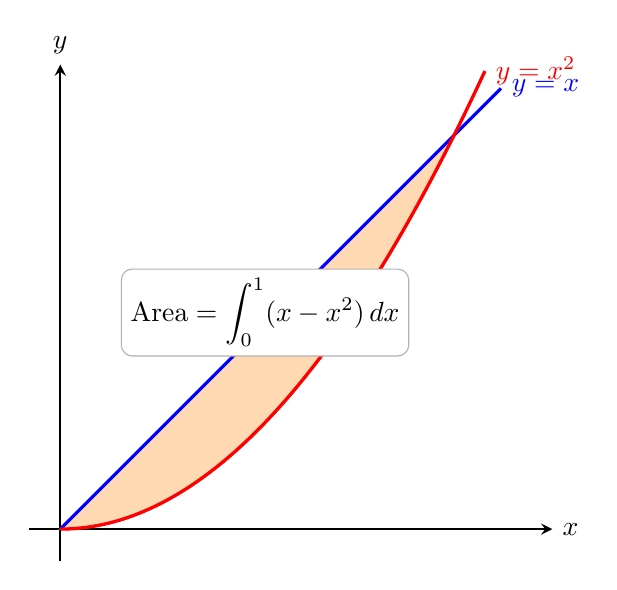
\begin{tikzpicture}[x=5cm,y=5cm,>=stealth]
\draw[->, thick] (-0.08,0) -- (1.25,0) node[right] {$x$};
\draw[->, thick] (0,-0.08) -- (0,1.18) node[above] {$y$};
\path[fill=orange!30, draw=orange!70!black, thick]
plot[domain=0:1,samples=100] (\x,{\x}) -- plot[domain=1:0,samples=100] (\x,{\x*\x}) -- cycle;
\draw[blue, very thick] plot[domain=0:1.12,samples=100] (\x,{\x}) node[right] {$y=x$};
\draw[red, very thick] plot[domain=0:1.08,samples=100] (\x,{\x*\x}) node[right] {$y=x^2$};
\node[align=center, fill=white, draw=black!30, rounded corners] at (0.52,0.55) {$\text{Area}=\displaystyle\int_0^1(x-x^2)\,dx$};
\end{tikzpicture}
\end{document}